\chapter{Basic data exploration}
\label{ch:basic_data_exploration}

\newthought{Let us consider another problem} Let us consider another problem, this time from clinical medicine. We will dig for something interesting in the data and explore it a bit with visualization widgets. You will get to know Quasar better, and also learn about several interesting visualizations.

We will start with an empty canvas; to clean it from our previous lesson, use either File/New or select all the widgets and remove them (use the backspace/delete key, or Cmd-backspace if you are on Mac).

Now again, add the File widget and open another documentation data set: heart\_disease. How does the data look like?

\begin{figure}[h]
  \centering
  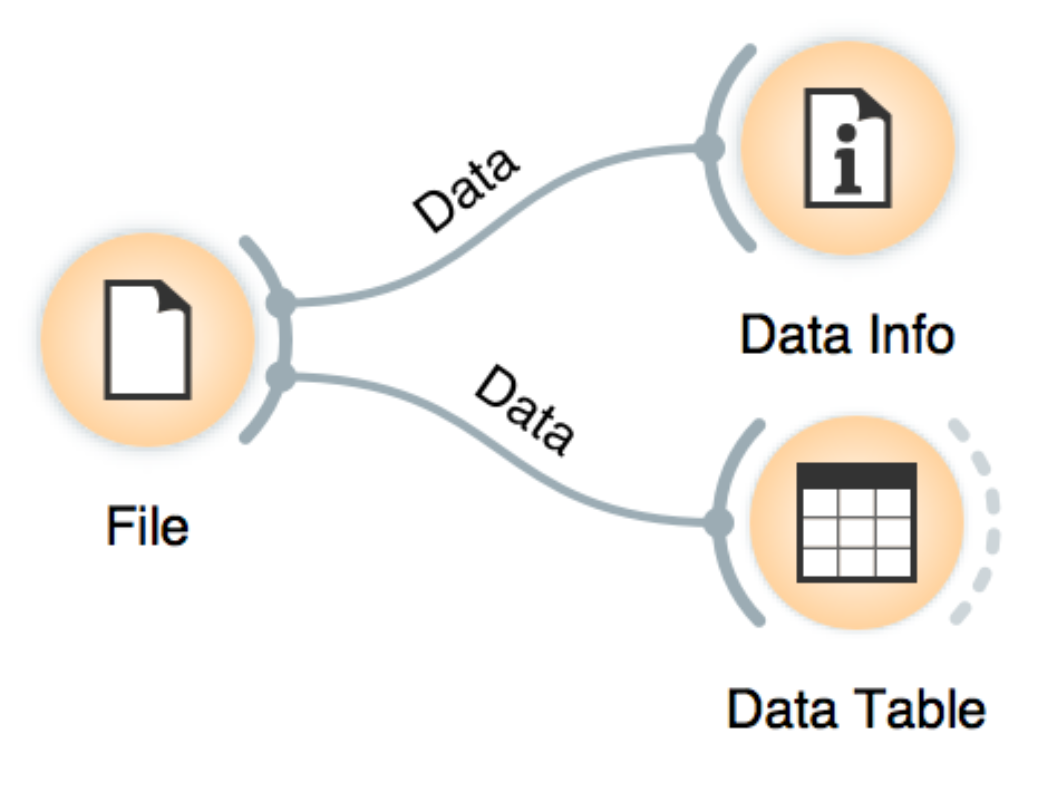
\includegraphics[width=50mm]{graphics/ch-basic_data_exploration/basic_data_exploration-fig1.png}%
  \caption{A simple workflow to inspect the loaded dataset.}
  \label{fig:basic_data_exploration-fig1}
\end{figure}

Let us check whether common visualizations tell us anything interesting. (Hint: look for gender differences. These are always interesting and occasionally even real.)

\begin{figure}[h]
  \centering
  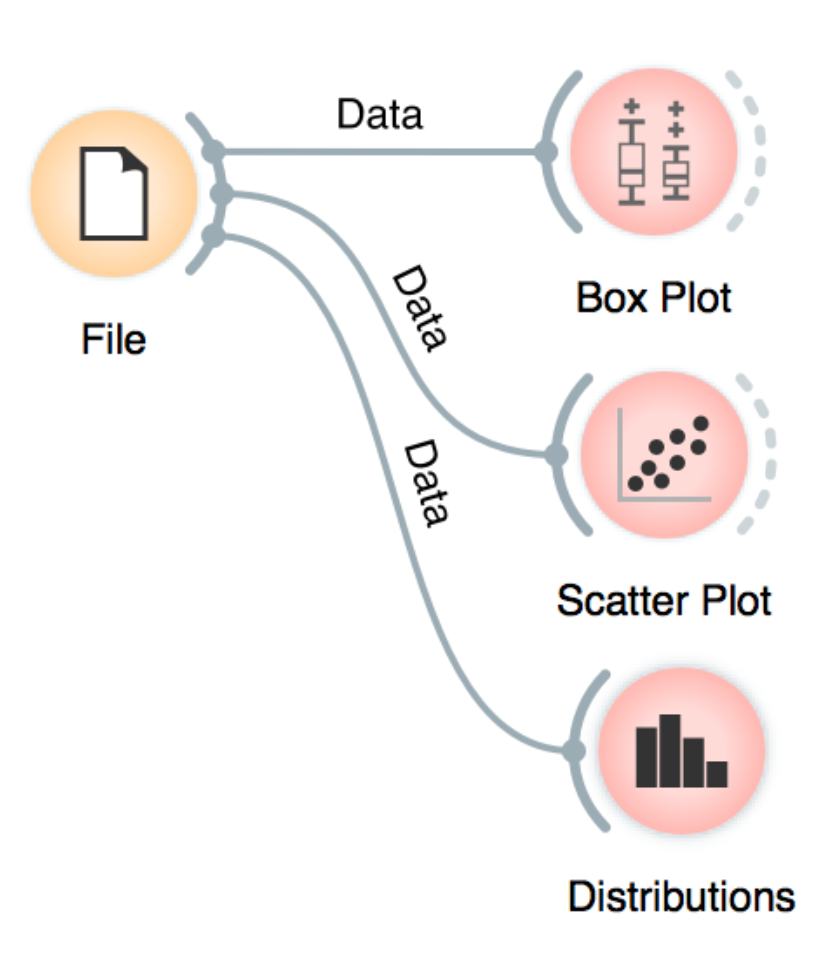
\includegraphics[width=50mm]{graphics/ch-basic_data_exploration/basic_data_exploration-fig2.png}%
  \caption{Quick check with common statistics and other visualization widgets.}
  \label{fig:basic_data_exploration-fig2}
\end{figure}

\newpage
Data can also be split by the value of features—in this case—the gender.

\begin{figure}[h]
  \centering
  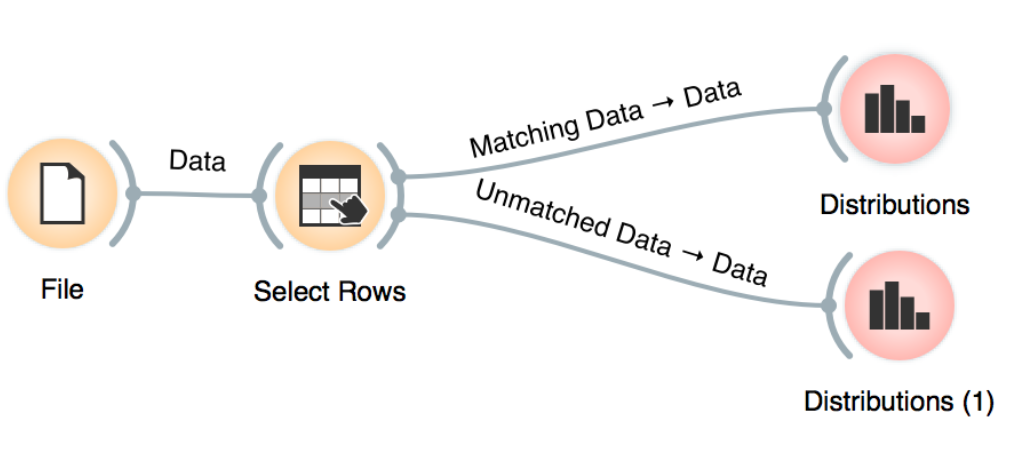
\includegraphics[width=90mm]{graphics/ch-basic_data_exploration/basic_data_exploration-fig3.png}%
  \caption{The two Distributions widgets get different data: the upper gets the selected rows and the lower gets the rest. Double-click the connection between the widgets to access setup dialog, as you've learned in the previous lesson.}
  \label{fig:basic_data_exploration-fig3}
\end{figure}

In the Select Rows widget, we select the female patients. You can also add other conditions. Selection of data instances provides a powerful combination with visualization of data distribution. Try having at least two widgets open at the same time and explore the data.

\begin{marginfigure}
%   \centering
  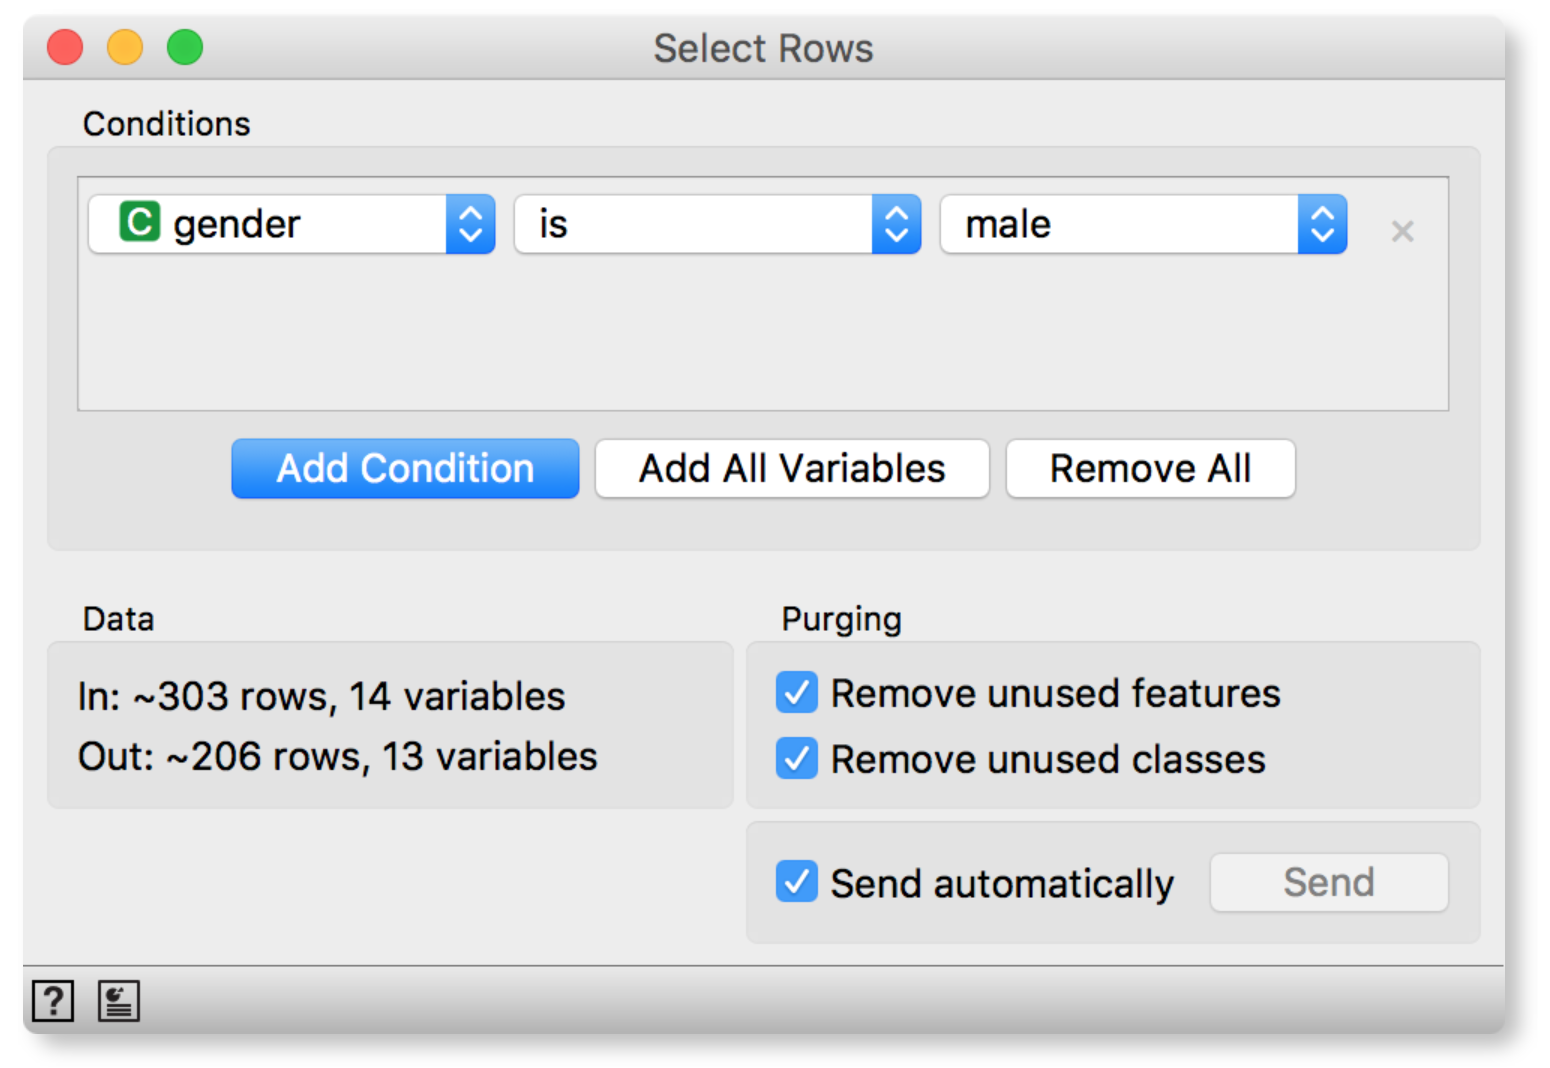
\includegraphics[width=\linewidth]{graphics/ch-basic_data_exploration/basic_data_exploration-fig4.png}%
  \caption{Select Rows and Distributions widget}
  \label{fig:basic_data_exploration-fig4}
\end{marginfigure}

\begin{figure*}[h]
%   \centering
  \flushright
  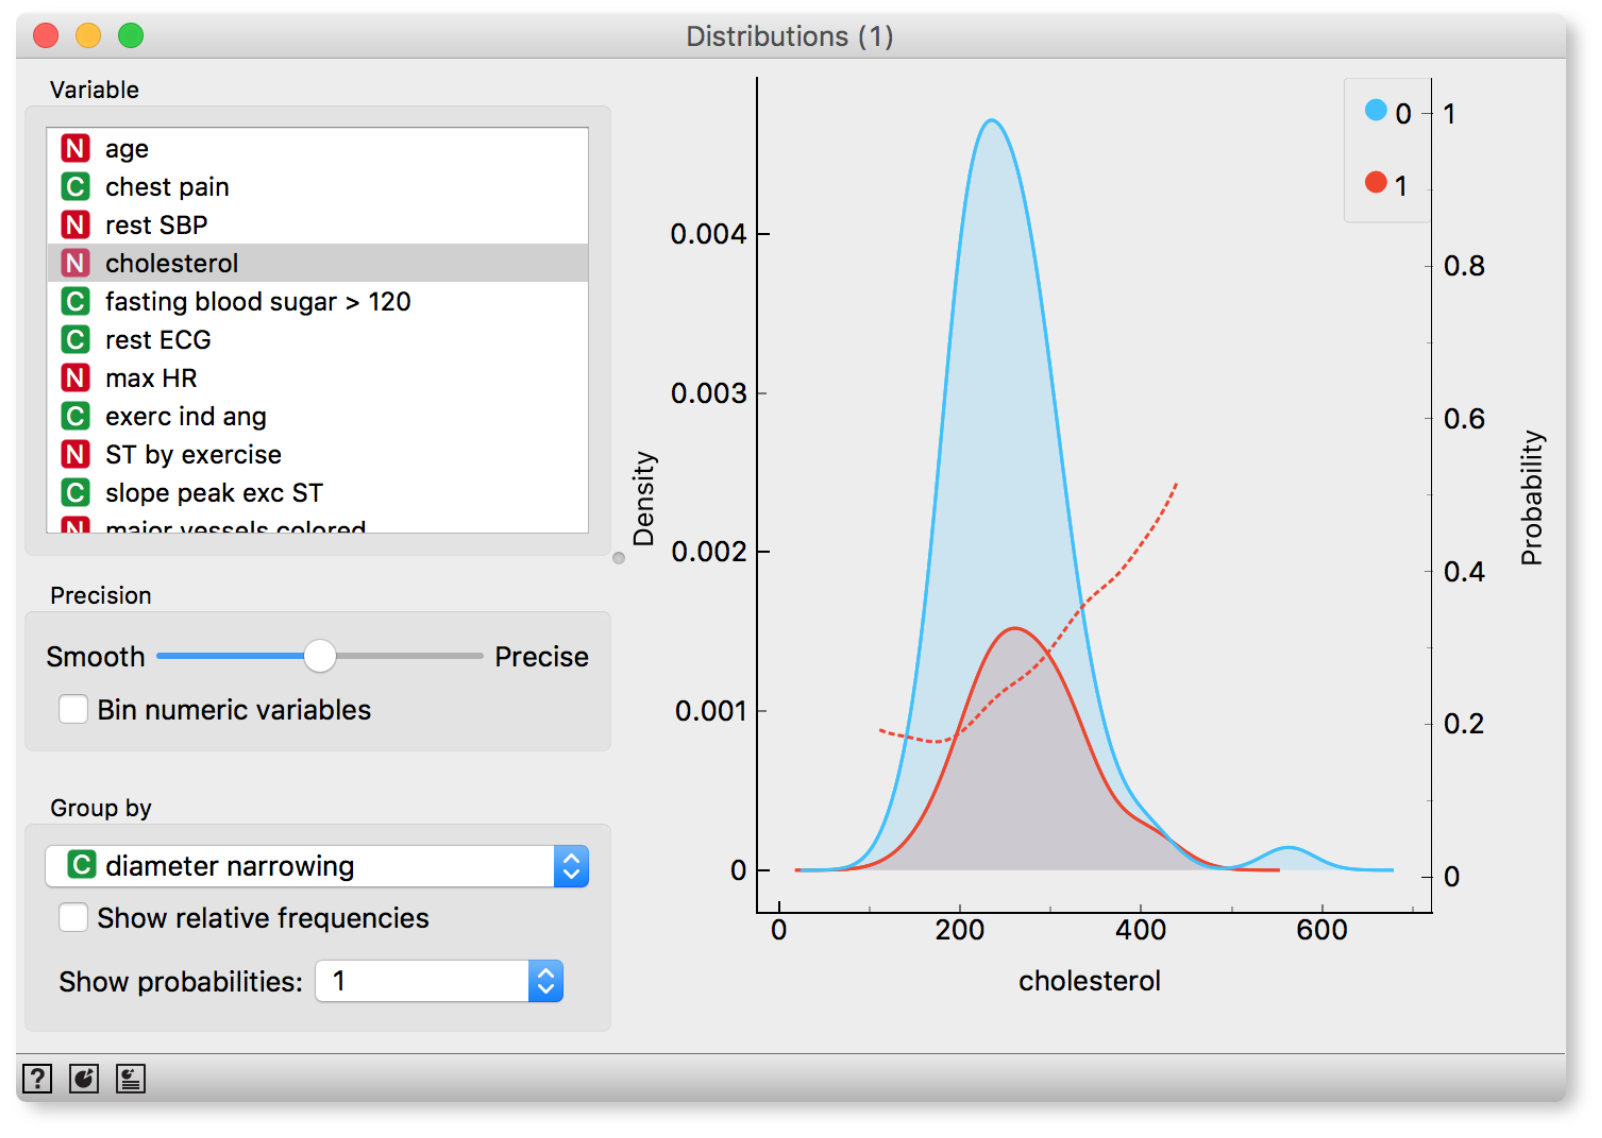
\includegraphics[width=115mm]{graphics/ch-basic_data_exploration/basic_data_exploration-fig5.png}
%   \caption{Scatter Plot and Ranking}
  \label{fig:basic_data_exploration-fig5}
\end{figure*}

There are two less known — but great — visualizations for observing interactions between features. 

Mosaic display shows a rectangle split into columns with widths reflecting the prevalence of different types of chest pain. Each column is then further split vertically according to gender distributions within the column. The resulting rectangles are split again horizontally according to age group sizes. Within the resulting bars, the red and blue areas represent the outcome distribution for each group and the tiny strip to the left of each shows the overall distribution.

\newpage
What can you read from this diagram?

\begin{figure}[h]
  \centering
  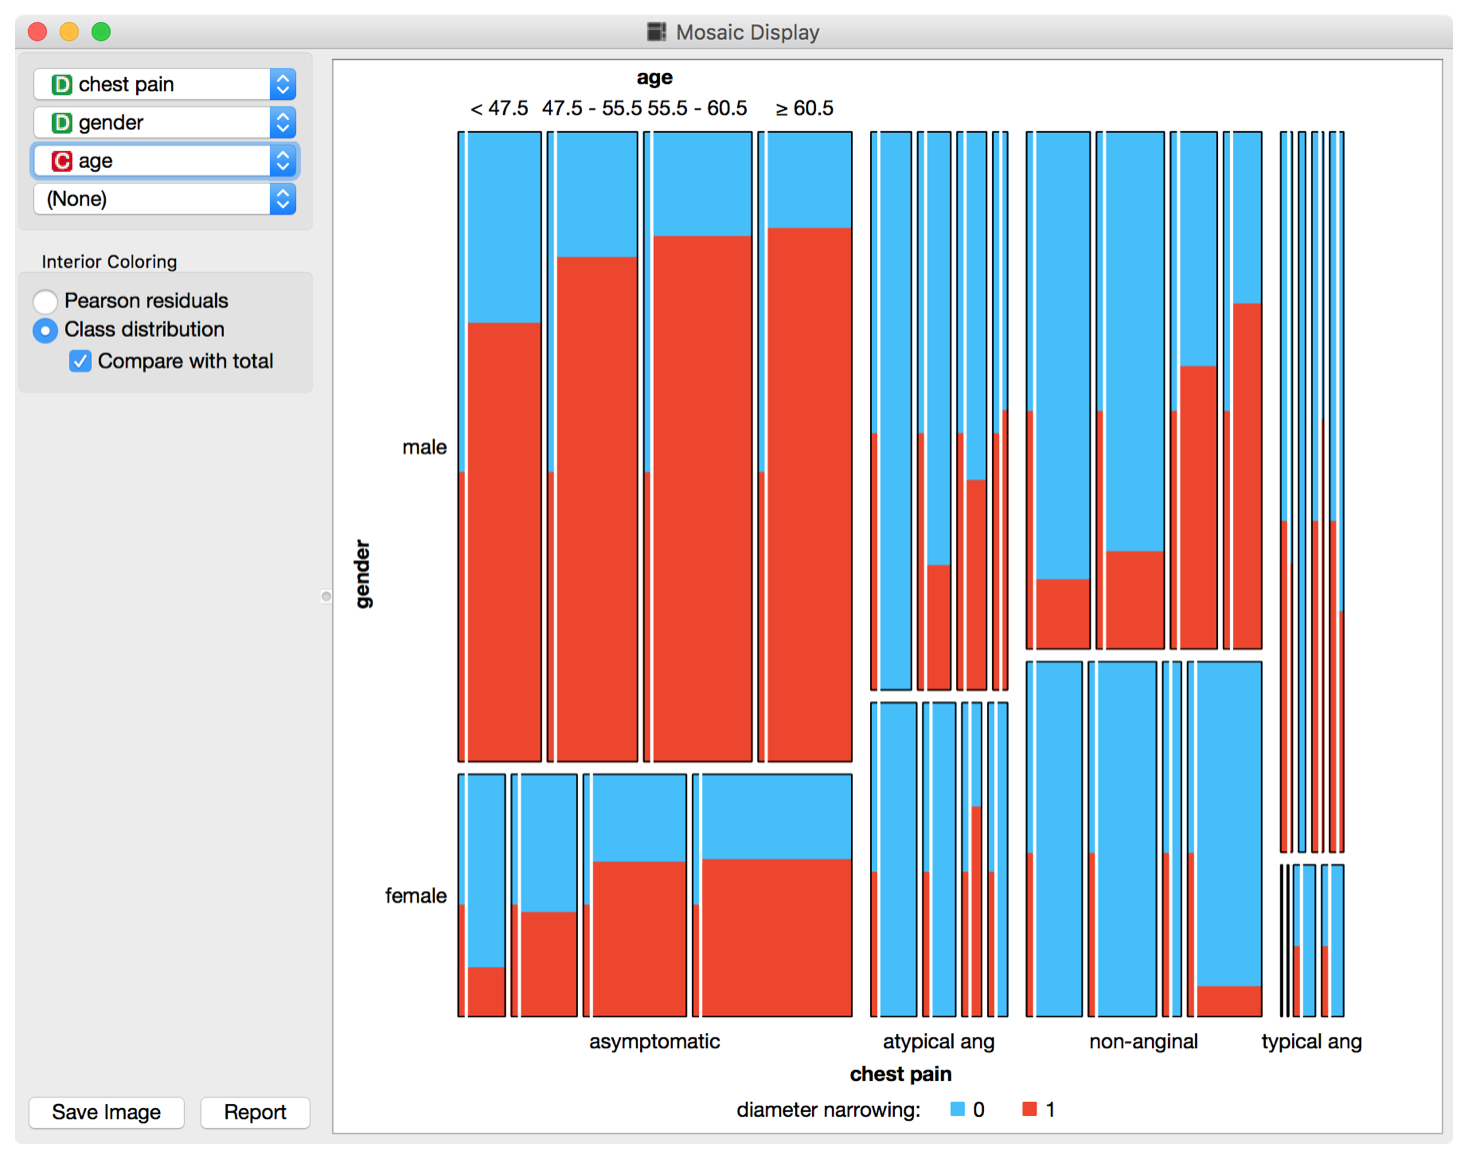
\includegraphics[width=\linewidth]{graphics/ch-basic_data_exploration/basic_data_exploration-fig6.png}
  \caption{You can play with the widget by trying different combinations of 1-4 features.}
  \label{fig:basic_data_exploration-fig6}
\end{figure}

Another visualization, Sieve diagram also splits a rectangle horizontally and vertically, but with independent cuts, so the areas correspond to the expected number of data instances if the observed variables were independent. For instance, 1/4 of patients are older than 60, and 1/3 of patients are female, so the area of the bottom right rectangle is 1/12 of the total area. With roughly 300 patients, we would expect 1/12 × 300 = 25 older women in our data. As a matter of fact, there are 34. Sieve diagram shows the difference between the expected and the observed frequencies by the grid density and the color of the field.

\begin{figure}
  \flushright
  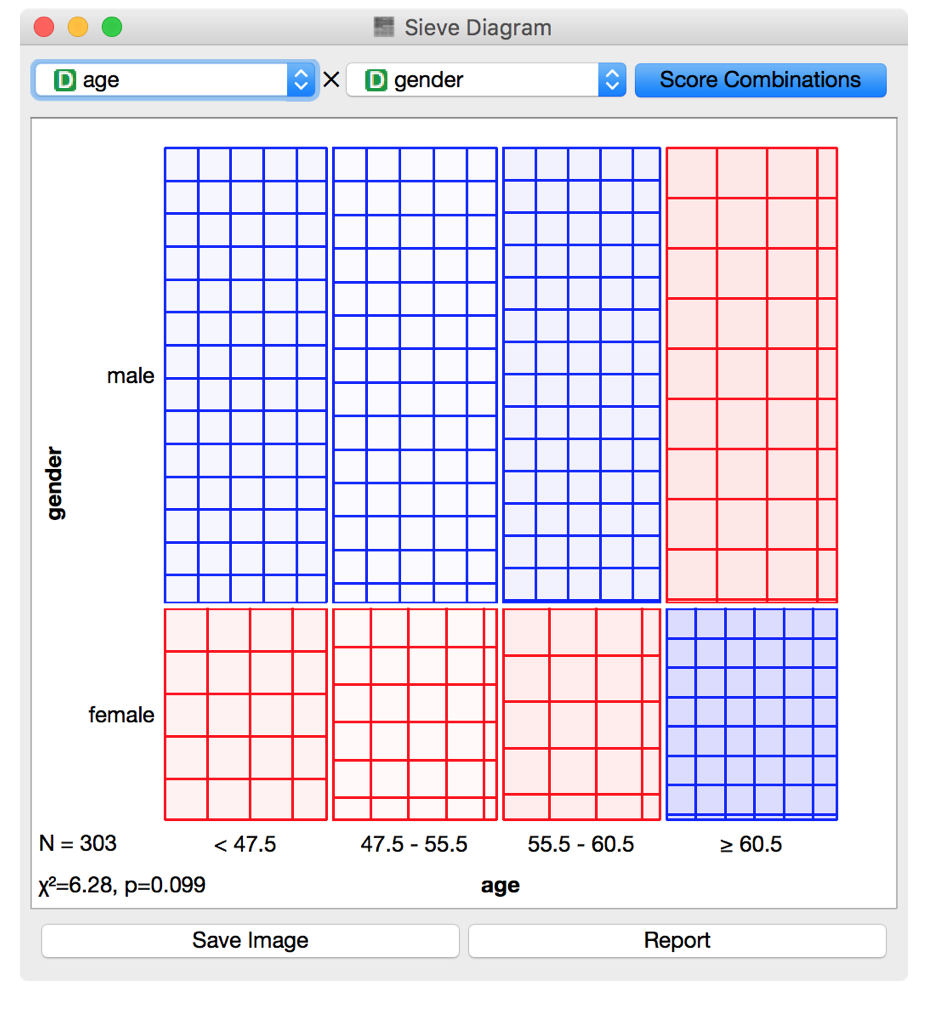
\includegraphics[width=70mm]{graphics/ch-basic_data_exploration/basic_data_exploration-fig7.png}
  \caption{See the Score Combinations button? Guess what it does? And how it scores the combinations? (Hint: there are some Greek letters at the bottom of the widget.)}
  \label{fig:basic_data_exploration-fig7}
\end{figure}